%
% CSE Electronic Homework Template
% Last modified 8/23/2018 by Jeremy Buhler

\documentclass[11pt]{article}
\usepackage[left=0.7in,right=0.7in,top=1in,bottom=0.7in]{geometry}
\usepackage{fancyhdr} % for header
\usepackage{graphicx} % for figures
\usepackage{amsmath}  % for extended math markup
\usepackage{amssymb}
\usepackage[bookmarks=false]{hyperref} % for URL embedding
\usepackage[noend]{algpseudocode} % for pseudocode
\usepackage[plain]{algorithm} % float environment for algorithms

%%%%%%%%%%%%%%%%%%%%%%%%%%%%%%%%%%%%%%%%%%%%%%%%%%%%%%%%%%%%%%%%%%%%%%
% STUDENT: modify the following fields to reflect your
% name/ID, the current homework, and the current problem number

% Example: 
%\newcommand{\StudentName}{Jeremy Buhler}
%\newcommand{\StudentID{123456}

\newcommand{\StudentName}{Ming-Che Teng}
\newcommand{\StudentID}{466303}
\newcommand{\HomeworkNumber}{6}

%%%%%%%%%%%%%%%%%%%%%%%%%%%%%%%%%%%%%%%%%%%%%%%%%%%%%%%%%%%%%%%%%%%%%%%%
% You can pretty much leave the stuff up to the next line of %%'s alone.

% create header and footer for every page
\pagestyle{fancy}
\fancyhf{}
\lhead{\textbf{\StudentName}}
\chead{\textbf{\StudentID}}
\rhead{\textbf{Assignment \HomeworkNumber}}
\cfoot{\thepage}

% preferred pseudocode style
\algrenewcommand{\algorithmicprocedure}{}
\algrenewcommand{\algorithmicthen}{}

% ``do { ... } while (cond)''
\algdef{SE}[DOWHILE]{Do}{doWhile}{\algorithmicdo}[1]{\algorithmicwhile\ #1}%

% ``for (x in y ... z)''
\newcommand{\ForRange}[3]{\For{#1 \textbf{in} #2 \ \ldots \ #3}}

% these are common math formatting commands that aren't defined by default
\newcommand{\union}{\cup}
\newcommand{\isect}{\cap}
\newcommand{\ceil}[1]{\ensuremath \left\lceil #1 \right\rceil}
\newcommand{\floor}[1]{\ensuremath \left\lfloor #1 \right\rfloor}
\newcommand*{\Perm}[2]{{}^{#1}\!P_{#2}}%
\newcommand*{\Comb}[2]{{}^{#1}C_{#2}}%
\newcommand*{\Int}{\int\limits}
\usepackage{listings}
\usepackage{color}


\definecolor{dkgreen}{rgb}{0,0.6,0}
\definecolor{gray}{rgb}{0.5,0.5,0.5}
\definecolor{mauve}{rgb}{0.58,0,0.82}
\lstset{frame=tb,
  language=Java,
  aboveskip=3mm,
  belowskip=3mm,
  showstringspaces=false,
  columns=flexible,
  basicstyle={\small\ttfamily},
  numbers=none,
  numberstyle=\tiny\color{gray},
  keywordstyle=\color{blue},
  commentstyle=\color{dkgreen},
  stringstyle=\color{mauve},
  breaklines=true,
  breakatwhitespace=true,
  tabsize=3
}

%%%%%%%%%%%%%%%%%%%%%%%%%%%%%%%%%%%%%%%%%%%%%%%%%%%%%%%%%%%%%%%%%%%%%%

\begin{document}
\subsection * {Problems}

\begin{enumerate}

\item [\textbf{1.}]  

Based on 3-nearest neighbor, the data point, $x = 3.2$, has $(3,5)$, $(3,8)$, and $(2,11)$ neighbors. By averaging the y value we can get, 

$$ g(x) = \frac{1}{3}\sum_{i=1}^{3}y_{[i]}(x) = 8$$


\item[\textbf{2.}]

The examples map from $[x_1, x_2]$ to $[x_1, x_1x_2]$ coordinates as follows:

$[-1, -1]$ (negative) maps to $[-1, +1]$

$[-1, +1]$ (positive) maps to $[-1, -1]$

$[+1, -1]$ (positive) maps to $[+1, -1]$

$[+1, +1]$ (negative) maps to $[+1, +1]$

In the parenthesis are XOR function. The positive examples have $x_1x_2 = -1$, the negative examples have $x_1x_2 = +1$. The maximum margin separator is the line $x_1x_2 0$, with the margin of 1. 

Transforming from $x_1, x_1x_2$ space back to $x_1, x_2$ the separator becomes either $x_1 = 0$ or $x_2 = 0$


\item[\textbf{3.}]

\begin{equation}
\begin{aligned}
K(x_i, x_j) =& \Phi(x_i)\Phi(x_j) \\
=& (\Phi(x_i)\ - Phi(x_j))^2\\
=& (\Phi(x_i))^2 - 2\Phi(x_i)\Phi(x_j)  + (\Phi(x_j))^2\\
=& K(x_i,x_i) + 2K(x_i,x_j) + K(x_j,x_j)
\end{aligned}
\end{equation}

Based on the equation above, we conclude that a kernel function, which is used to compute squared Euclidean distance in the projected space, can be simplified to compute dot product of two transformed dimensions. 

\end{enumerate}

\subsection*{Problem}
\begin{enumerate}

\item[\textbf{4.}]

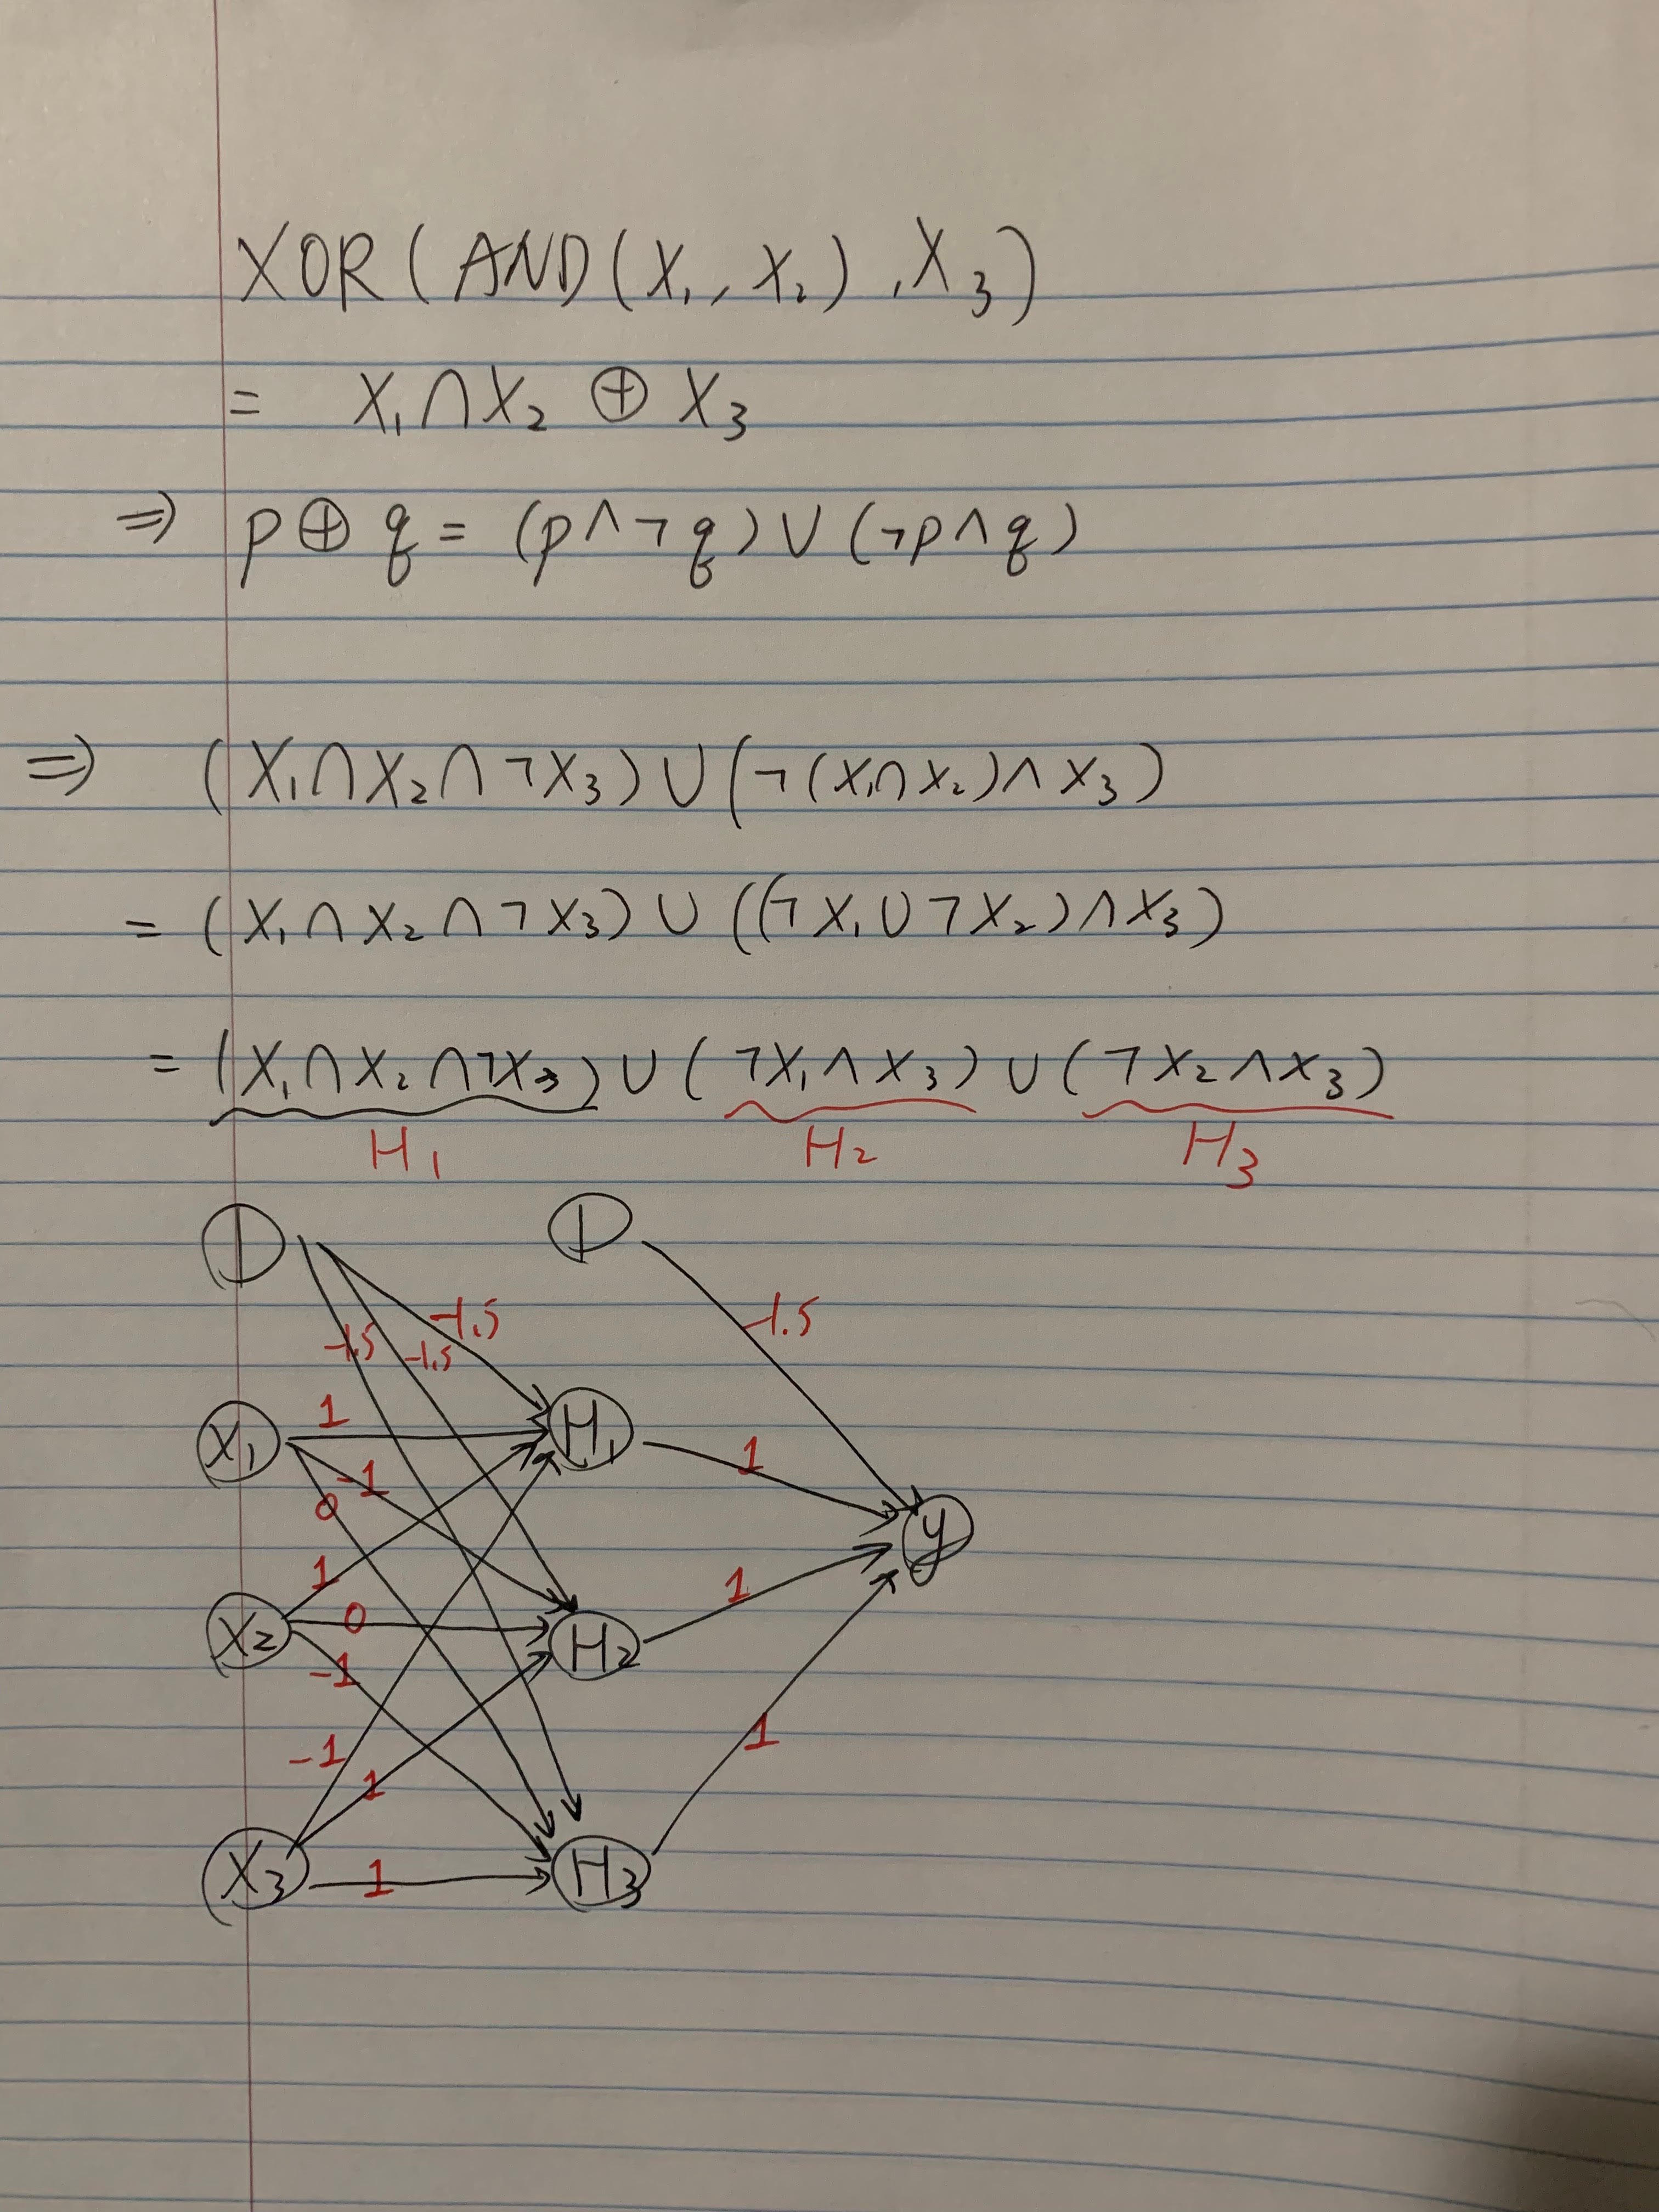
\includegraphics[scale = 0.15]{/Users/alexteng/Desktop/CSE417/H6_4.jpg}





\end{enumerate}
\pagebreak


\subsection*{Collaboration Statement}

I didn't collaborate with anyone for this assignment.

\end{document}